\section{Hazard Scenario Selection}
    In this section, the critical task of selecting an appropriate hazard scenario is explored, a decision that profoundly shapes community resilience strategies. Three hypothetical resilience actions are introduced, each tailored to address specific vulnerabilities, and their impact is analyzed using separate loss functions. The focus lies in understanding the probability of different damage states after the application of each resilience action and evaluating their benefits against implementation costs. This exploration underscores the strategic importance of hazard scenario selection, guiding informed decisions crucial for resilient communities. The diverse set of samples generated in the previous section will be leveraged to conduct comprehensive comparisons, shedding light on the effectiveness of various hazard scenarios.

    The three hypothetical resilience actions are exemplified as follows:
    \begin{itemize}
        \item \textbf{Resilience Action 1 - Community Education and Preparedness Programs}: Launching community-wide education initiatives to raise awareness about disaster preparedness, equipping residents with essential skills and knowledge to cope with emergencies effectively.
        \item \textbf{Resilience Action 2 - Early Warning Systems}: Implementing advanced early warning systems to alert residents about imminent hazards, enabling timely evacuation and preparedness.
        \item \textbf{Resilience Action 3 - Infrastructure Reinforcement}: Strengthening critical infrastructure such as buildings, bridges, and utility systems to withstand natural disasters, reducing potential damage and ensuring continuity of essential services.
    \end{itemize}

    The corresponding loss functions for these actions, reflecting the expected loss under various hazard scenarios, are visually depicted in Fig.~\ref{fig:loss_functions}.

        \begin{figure}[H]
        \centering
        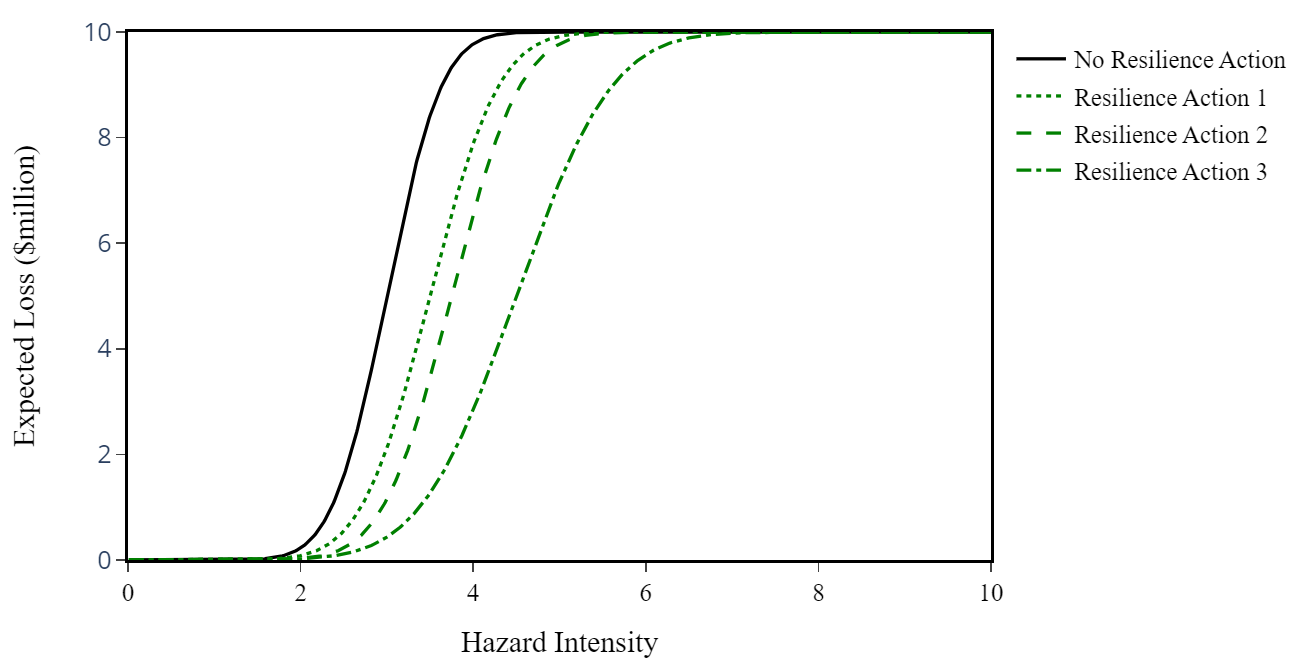
\includegraphics[scale=0.5]{Figures/Images/Hazard Scenario Selection/loss_functions.png}
        \caption{Visual representation of the loss functions associated with the hypothetical resilience actions}
        \label{fig:loss_functions}
    \end{figure}
    
    Each resilience action in Fig.~\ref{fig:loss_functions} demonstrates a distinct reduction in expected losses as hazard intensity increases, highlighting the complex interplay between resilience strategies and their associated costs.

    In the initial phase of the analysis, we set specific thresholds to evaluate the chance of different damage states occurring after implementing resilience actions. These thresholds are \$3 million for minor damage, \$5 million for moderate damage, and \$7 million for extensive damage. These thresholds will be utilized to compare the hazard scenarios generated from different simulation methods discussed in the previous section, determining the probability of surpassing each damage state under distinct resilience actions. This section compares three simulation methods: MC simulation, manual-IS, and MCMC-IS techniques. The corresponding exceedance probability curves for these methods are illustrated in Fig.~\ref{fig:exceedance_probabilities}. In this hypothetical situation, stakeholders can evaluate the effectiveness of various resilience actions under different hazard scenarios.
    
        \begin{figure}[H]
        \centering
        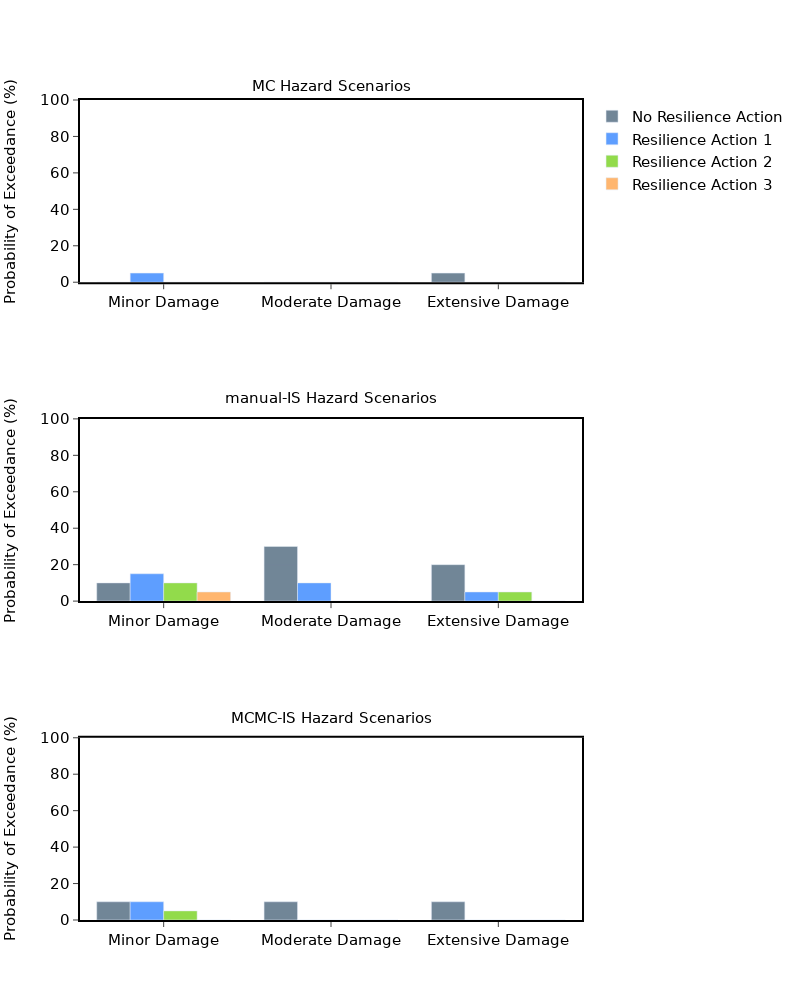
\includegraphics[scale=0.4]{Figures/Images/Hazard Scenario Selection/exceedance_probabilities.png}
        \caption{Comparison of exceedance probabilities for different damage states under various resilience actions across distinct hazard scenarios}
        \label{fig:exceedance_probabilities}
    \end{figure}

    Fig.~\ref{fig:exceedance_probabilities} shows the diversity in the probability of exceedance values among scenarios generated by the three simulation methods using the same number of scenarios. This contrast highlights the profound impact of selecting accurate hazard scenarios and the necessity of employing sophisticated simulation methods, like MCMC-IS, which capture intricate risk factors more comprehensively.

    Furthermore, we employed a straightforward cost-benefit approach to assess the effectiveness of different resilience actions under the generated hazard scenarios. To identify the most advantageous resilience action for each set of hazard scenarios, we calculated the net benefit of each action, considering the reduction in losses associated with its implementation. The associated implementation costs for the three resilience actions are presented in Table~\ref{table:implementation_costs}. \\
        
    \begin{table}[H]
    \centering
    \caption{Hypothetical implementation costs for resilience actions}
    \label{table:implementation_costs}
    \begin{tabular}{lc}
        \hline
        \textbf{Resilience Action} & \textbf{Implementation Cost} (\$ million) \\
        \hline
        1 - Community Education Programs & 1 \\
        2 - Early Warning Systems & 2 \\
        3 - Infrastructure Reinforcement & 5 \\
        \hline
    \end{tabular}
\end{table}

    
    In Table \ref{tab:cost_benefit}, the benefits associated with different resilience actions under various simulation methods are outlined. The selection of the resilience action for each method was determined based on the maximum benefit criterion. A negative benefit indicates the infeasibility of the corresponding resilience action, signifying that implementing such actions would result in higher losses compared to having no resilience measures in place.
        
    \begin{table}[h]
    \centering
    \caption{Benefits (in \$million) of different resilience actions}
    \begin{tabular}{lccc}
        \hline
        \textbf{Method} & \textbf{Resilience Action 1} & \textbf{Resilience Action 2} & \textbf{Resilience Action 3} \\ \hline
        \textbf{MC} & -0.078 & -0.783 & -3.634 \\ 
        \textbf{manual-IS} & 1.306 & 1.138 & -1.063 \\ 
        \textbf{MCMC-IS} & 0.663 & 0.214 & -2.424 \\ \hline
    \end{tabular}
    \label{tab:cost_benefit}
\end{table}


    Upon analyzing the results, it was observed that for the MC simulation method, all resilience actions resulted in negative benefits, indicating that none of these measures were feasible. Conversely, when evaluating the results from Manual-IS and MCMC-IS techniques, Resilience Action 1 and Resilience Action 2 showed positive benefits, with Resilience Action 1 being the preferred option in MCMC-IS due to its higher benefit. This discrepancy between the methods highlights the importance of selecting the appropriate simulation technique to accurately represent hazard scenarios, thereby facilitating more informed decision-making in resilience planning.
    